\hypertarget{_s_q_problem_8cpp}{}\section{/home/zheng/catkin\+\_\+ws/src/qp\+O\+A\+S\+E\+S-\/3.2.1/src/\+S\+Q\+Problem.cpp File Reference}
\label{_s_q_problem_8cpp}\index{/home/zheng/catkin\+\_\+ws/src/qp\+O\+A\+S\+E\+S-\/3.\+2.\+1/src/\+S\+Q\+Problem.\+cpp@{/home/zheng/catkin\+\_\+ws/src/qp\+O\+A\+S\+E\+S-\/3.\+2.\+1/src/\+S\+Q\+Problem.\+cpp}}
{\ttfamily \#include $<$qp\+O\+A\+S\+E\+S/\+S\+Q\+Problem.\+hpp$>$}\newline
Include dependency graph for S\+Q\+Problem.\+cpp\+:
\nopagebreak
\begin{figure}[H]
\begin{center}
\leavevmode
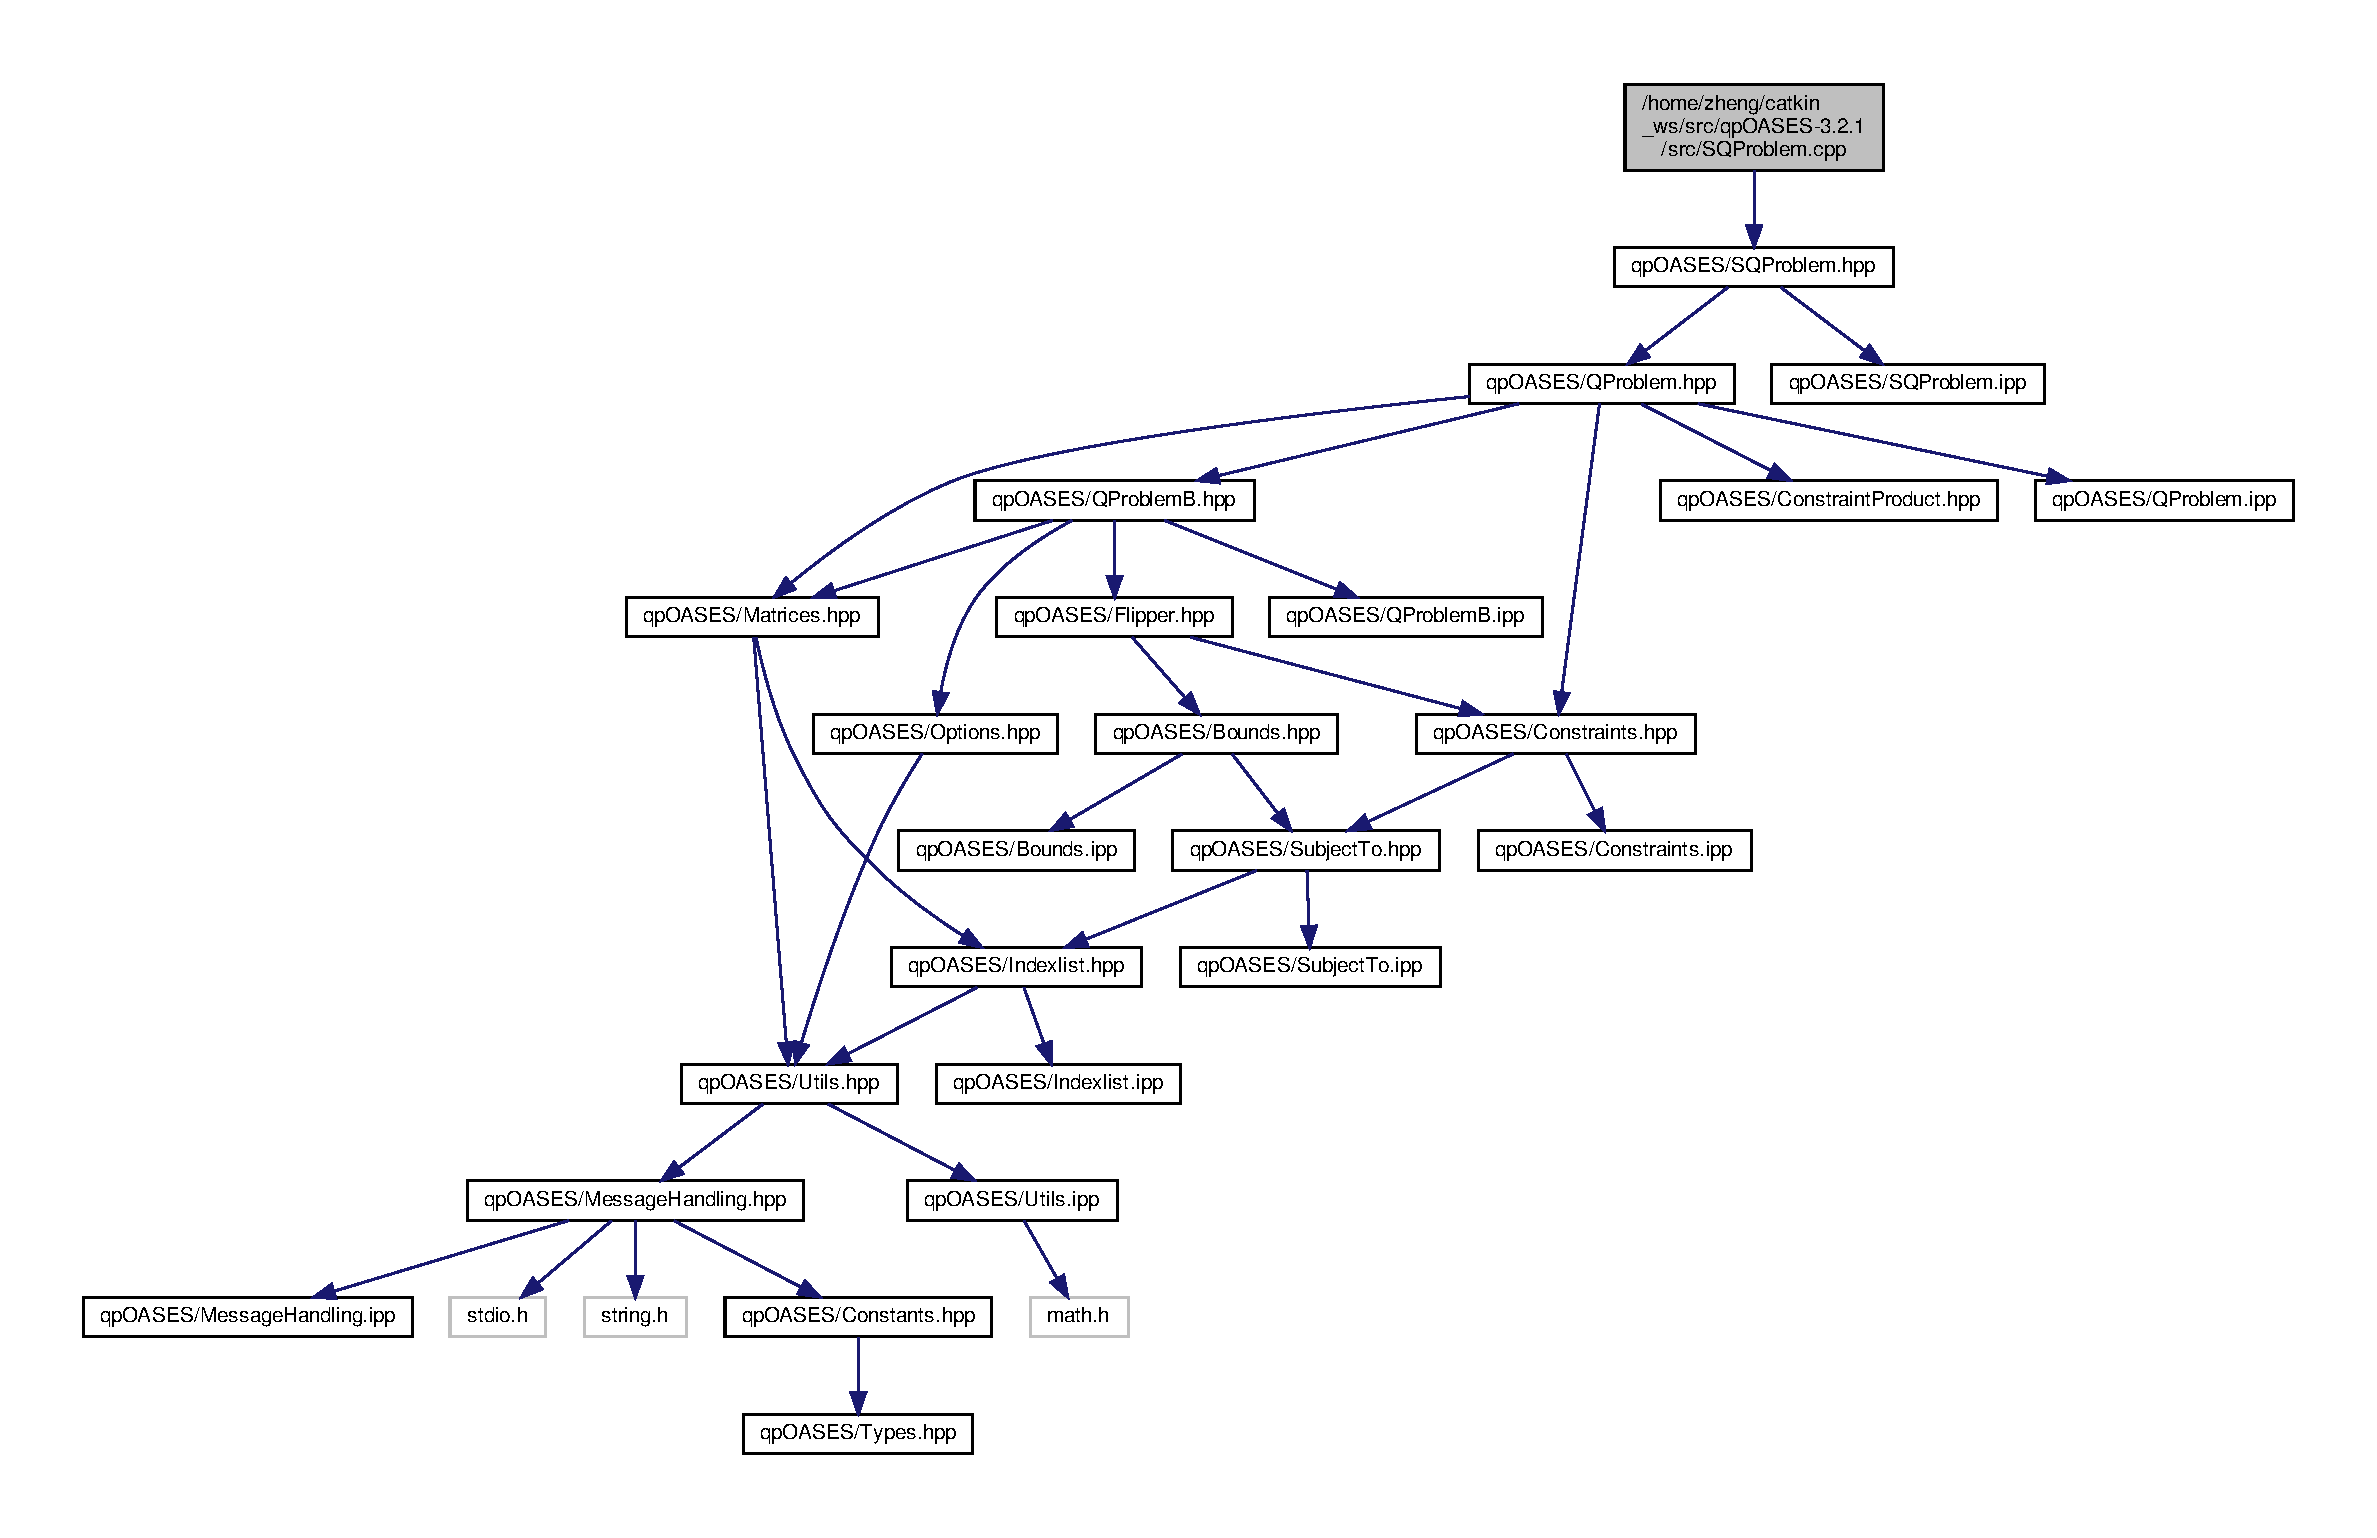
\includegraphics[width=350pt]{_s_q_problem_8cpp__incl}
\end{center}
\end{figure}


\subsection{Detailed Description}
\begin{DoxyAuthor}{Author}
Hans Joachim Ferreau, Andreas Potschka, Christian Kirches 
\end{DoxyAuthor}
\begin{DoxyVersion}{Version}
3.\+2 
\end{DoxyVersion}
\begin{DoxyDate}{Date}
2007-\/2017
\end{DoxyDate}
Implementation of the \hyperlink{class_s_q_problem}{S\+Q\+Problem} class which is able to use the newly developed online active set strategy for parametric quadratic programming with varying matrices. 